\documentclass{beamer}

  \mode<presentation> {
    \usetheme{Madrid}
    % \usecolortheme{seagull}
  }
  
  \usepackage{pscyr}
  \usepackage[T2A]{fontenc}
  \usepackage[utf8]{inputenc}
  \usepackage[english, russian]{babel}
  \usepackage{graphicx}
  \usepackage{booktabs}
  \usepackage{amsmath,amsfonts,amssymb,amsthm,mathtools}
  \usepackage{euscript}
  \usepackage{mathrsfs}

  %----------------------------------------------------------
  %   META
  %----------------------------------------------------------



  \title[Аппроксимация стабильного моста]{Задача аппроксимации максимального стабильного моста в позиционных дифференциальных играх}  
  \author{Кощеев Никита}
  \institute[УрФУ]{Институт естественных наук и математики}
  \date{15 июня 2018}

  \mathtoolsset{showonlyrefs=true}
  \graphicspath{ {images/} }


  \renewcommand{\rmdefault}{ftm}
  \newcommand{\dimension}{\mathbb{R}^2}


  %----------------------------------------------------------------------------------------
  %   TITLE PAGE
  %----------------------------------------------------------------------------------------
  
  \begin{document}
  
  \begin{frame}
      
    \titlepage 
    
  \end{frame}
  
  % \begin{frame}
  % \frametitle{Overview} 
  % \tableofcontents 
  % \end{frame}
  
  %----------------------------------------------------------------------------------------
  %   PRESENTATION SLIDES
  %----------------------------------------------------------------------------------------
  
  \begin{frame}
    \frametitle{Пример игры}
  
    \begin{equation}
        \frac{dx}{dt} = u + v, u \in P, v \in Q
    \end{equation}

    $M \subset \dimension$ - Терминальное(целевое) множество 
    \vspace{5mm}
  
    $\theta$ - момент окончания игры

    Цель первого игрока: обеспечить $x(\theta) \in M$

    Цель второго игрока: обеспечить $x(\theta) \notin M$

  \end{frame}

  

  %------------------------------------------------

  \begin{frame}
    \frametitle{Стабильный мост}

    $W \in [t_0, \theta] \times \dimension$ - стабильный мост

    $W(\theta)=R$

    \begin{itemize}
      \item Применение оптимального управления первым игроком,
      при $x_0 \in W(t_0)$ гарантирует $x(\theta) \in R$
      \item Применение оптимального управления вторым игроком,
      при $x_0 \notin W(t_0)$ гарантирует $x(\theta) \notin R$
    \end{itemize}

  \end{frame}
  
  %------------------------------------------------
  
  \begin{frame}
    \frametitle{Терминальное множество}
    
    Замкнутое множество в пространстве $\dimension$

    \begin{block}{Типы терминальных множеств}
      \begin{itemize}
        \item произвольный невыпуклый многоугольник
        \item многоугольник содержащий внутри себя отверстие
        \item множество произвольных многоугольников содержащих произвольное число отверстий
      \end{itemize}
    \end{block}

  \end{frame}
  
   %------------------------------------------------

   \subsection{CGAL} 
  
   \begin{frame}
     \frametitle{CGAL}
     
\includegraphics[width=1.0\textwidth]{cgal-logo}
 
     The Computational Geometry Algorithms Library
 
     Компоненты:
 
     \begin{itemize}
         \item 2D and 3D Linear Geometry Kernel
         \item 2D Polygons
         \item 2D Minkowski Sums
         \item 2D Polyline Simplification
     \end{itemize}
 
    \end{frame}


  %------------------------------------------------
  
  \begin{frame}
    \frametitle{Алгебраическая сумма}
    
    Другое название - "сумма Минковского". 
    
    \begin{equation}
      A \oplus B =  \{ x + y | x \in A, y \in B \} 
    \end{equation}

    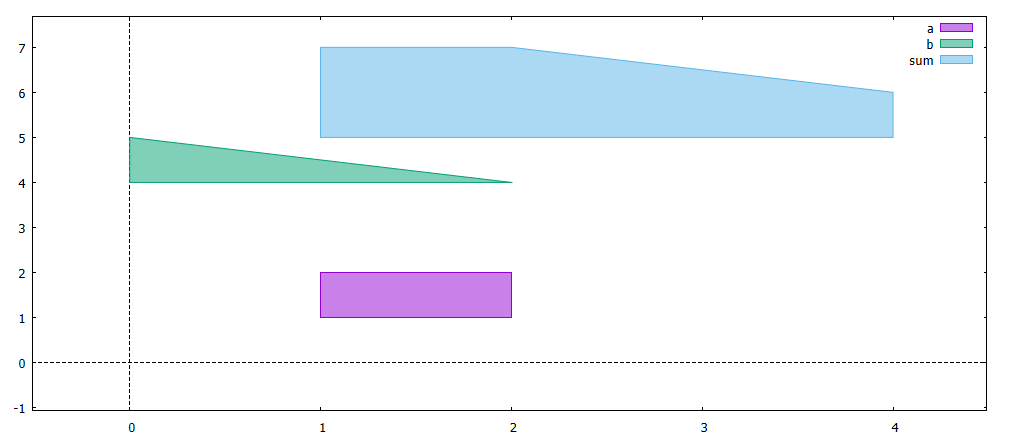
\includegraphics[width=1.0\textwidth]{sum}
  
  \end{frame}
  
  %------------------------------------------------
  
  \begin{frame}
    \frametitle{Геометрическая разность}
    
    \begin{equation}
      A \ominus B =  \{ x | x + B \subseteq A \} 
    \end{equation}

    \begin{equation}
        A \ominus B =
        (\overline{\overline{A} \oplus (- B)})
    \end{equation}  

    \begin{figure}
        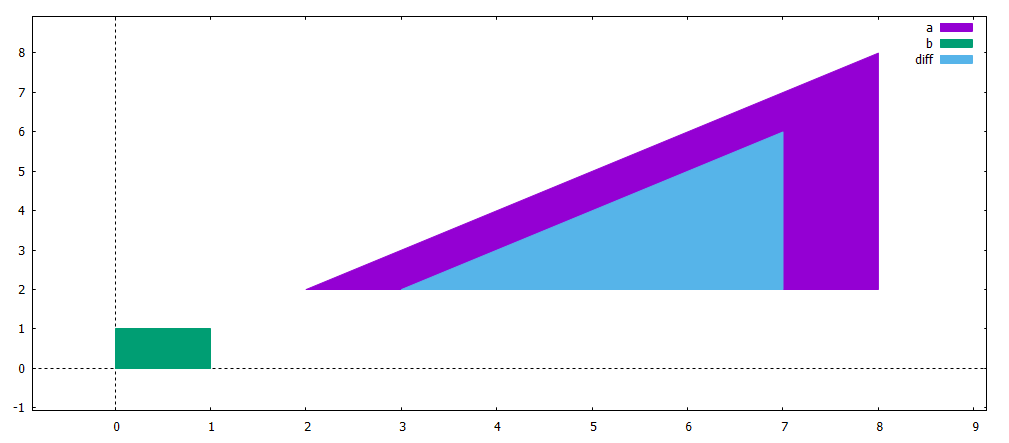
\includegraphics[scale=0.4]{diff}
    \end{figure}

  \end{frame}
  
  %------------------------------------------------
  
  \begin{frame}
    \frametitle{Упрощение множеств}

    \begin{figure}
        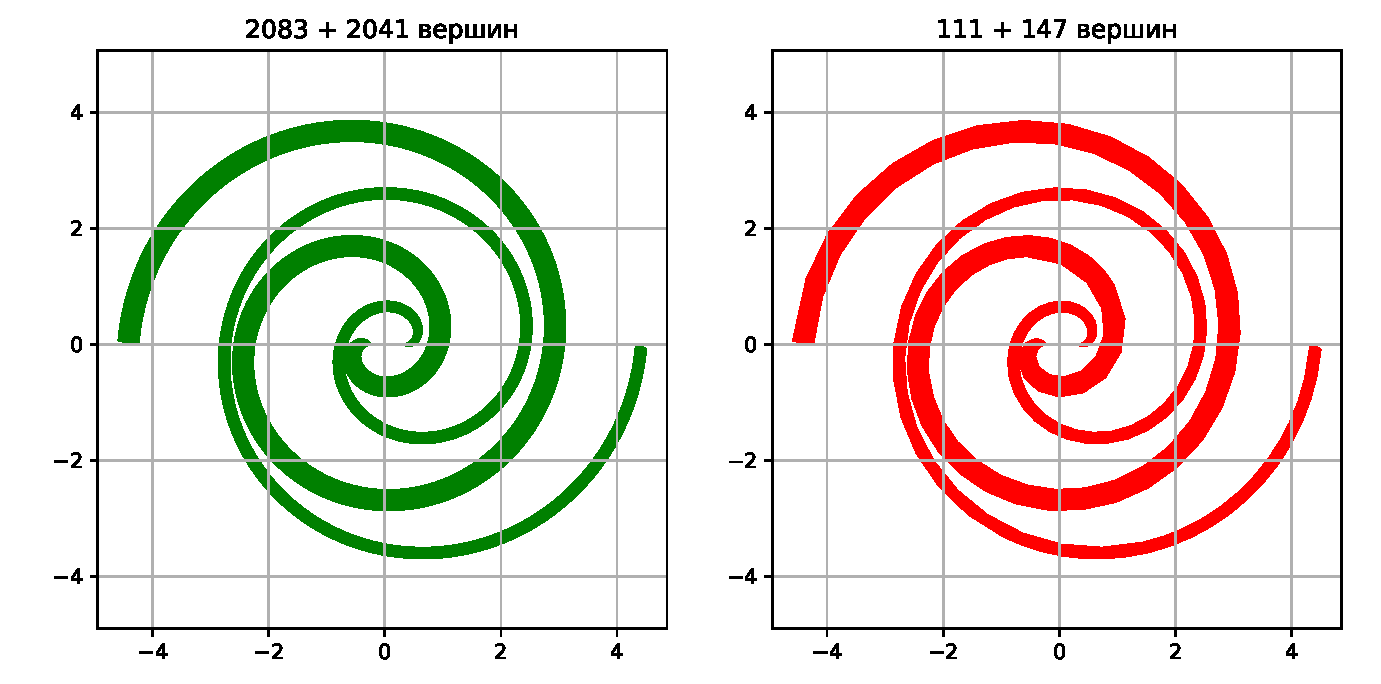
\includegraphics[width=1.0\textwidth]{spiral_simple}
    \end{figure}

  \end{frame}


  %------------------------------------------------ 

  \begin{frame}
    \frametitle{Удаление вершин}

    \begin{figure}
        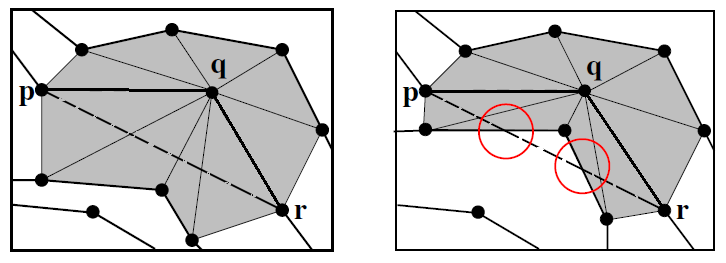
\includegraphics[width=1.0\textwidth]{platelet}
    \end{figure}

  \end{frame}

  %------------------------------------------------ 

  
  \begin{frame}
    \frametitle{Пример задачи}

    \begin{block}{Условия}
      \begin{itemize}
        \item $\theta = 10 с$ - момент окончания

        \item $\Delta t = 0.2$ - шаг разбиения $\{t_i\}, t_n = \theta$

        \item $P$, $Q$ - возможные управления игроков

        \item $M$ - терминальное множество

      \end{itemize}
    \end{block}

    \begin{block}{Хотим получить}
      Набор \textit{t}-сечений стабильного моста $\{W_{i}\}$  
    \end{block}

    \begin{block}{Формула}
      $W_0 = M$

      $W_{i+1} = ( W_i \oplus P ) \ominus  Q$
    \end{block}

  \end{frame}

  \begin{frame}
    \frametitle{Задача сближения-уклонения}

    \begin{figure}
        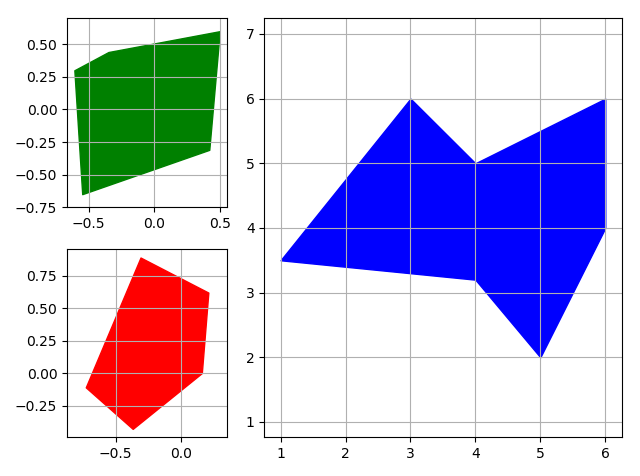
\includegraphics[width=\linewidth,height=0.8\textheight,keepaspectratio]{example1_pqm}
    \end{figure}

  \end{frame}  

  %----------------------------------------------------------------------------------------

  \begin{frame}
    \frametitle{Задача сближения-уклонения мост спереди}

    \begin{figure}
        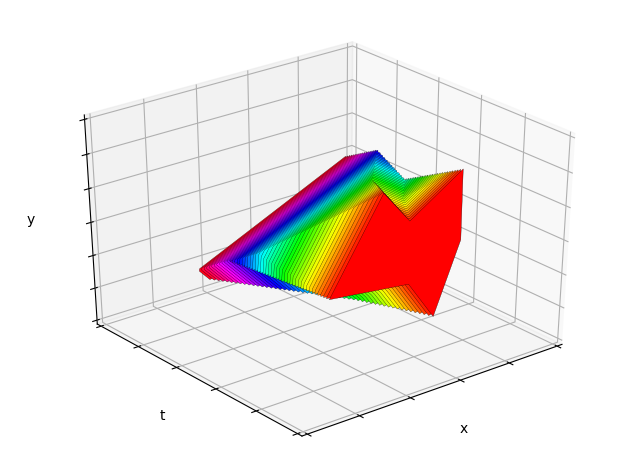
\includegraphics[width=\linewidth,height=0.8\textheight,keepaspectratio]{example1_bridge_front}
    \end{figure} 

  \end{frame}

  %----------------------------------------------------------------------------------------

  \begin{frame}
    \frametitle{Задача сближения-уклонения мост сзади}

    \begin{figure}
        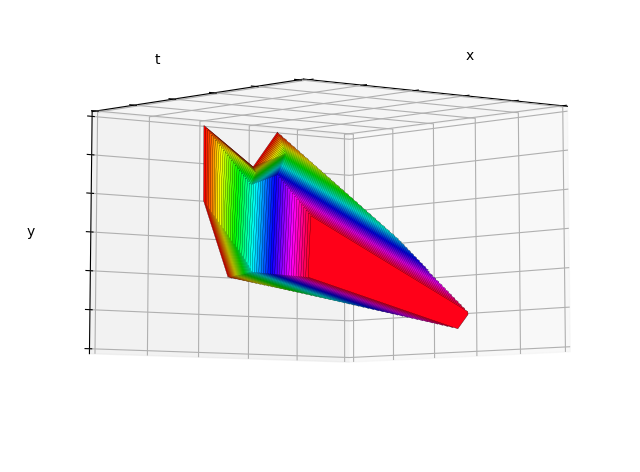
\includegraphics[width=\linewidth,height=0.8\textheight,keepaspectratio]{example1_bridge_back}
    \end{figure} 

  \end{frame}

  %----------------------------------------------------------------------------------------

  \begin{frame}
    \frametitle{Задача наблюдения}

    \begin{figure}
        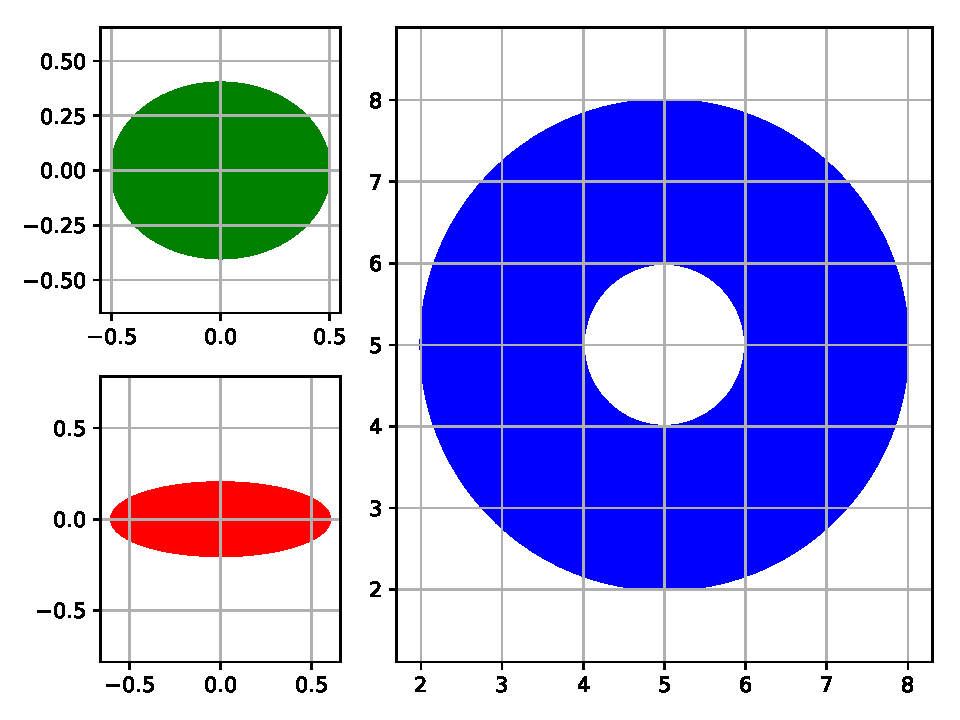
\includegraphics[width=\linewidth,height=0.8\textheight,keepaspectratio]{example2_pqm}
    \end{figure}

  \end{frame}  

  %----------------------------------------------------------------------------------------

  \begin{frame}
    \frametitle{Задача наблюдения мост спереди}

    \begin{figure}
        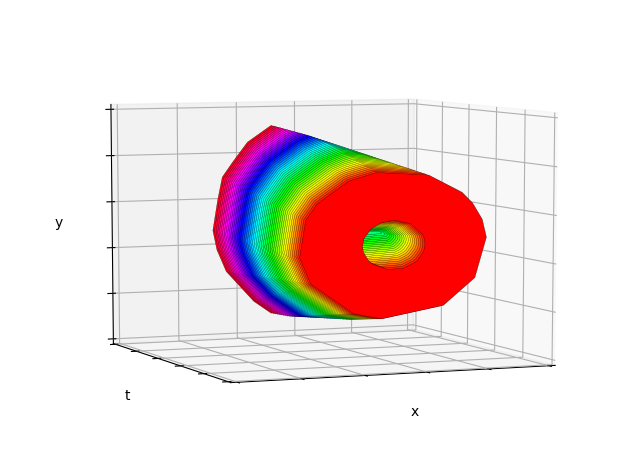
\includegraphics[width=\linewidth,height=0.8\textheight,keepaspectratio]{example2_bridge_front}
    \end{figure} 

  \end{frame}

  %----------------------------------------------------------------------------------------

  \begin{frame}
    \frametitle{Задача наблюдения мост сзади}

    \begin{figure}
        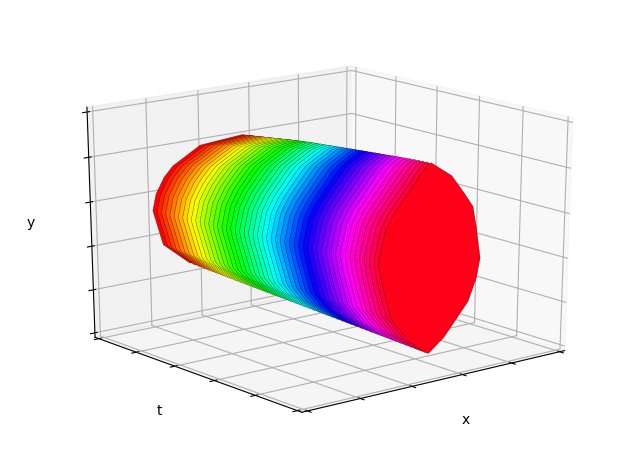
\includegraphics[width=\linewidth,height=0.8\textheight,keepaspectratio]{example2_bridge_back}
    \end{figure} 

  \end{frame}


  %----------------------------------------------------------------------------------------

  \begin{frame}
    \frametitle{Задача со сложным терминальным множеством}

    \begin{figure}
        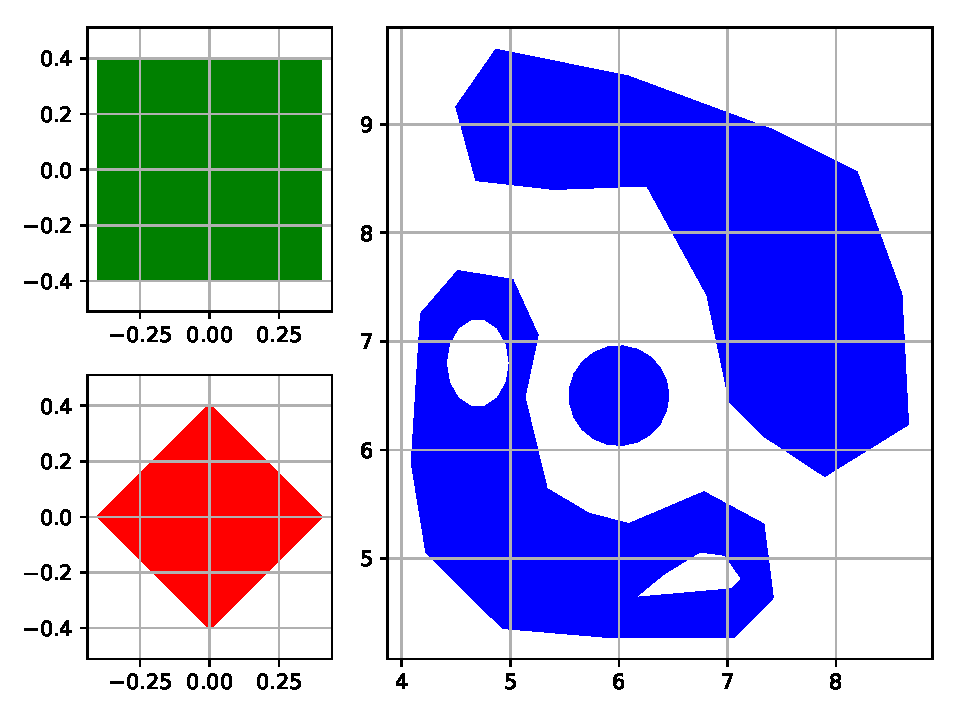
\includegraphics[width=\linewidth,height=0.8\textheight,keepaspectratio]{example3_pqm}
    \end{figure}

  \end{frame}  

  %----------------------------------------------------------------------------------------

  \begin{frame}
    \frametitle{Задача со сложным терминальным множеством мост спереди}

    \begin{figure}
        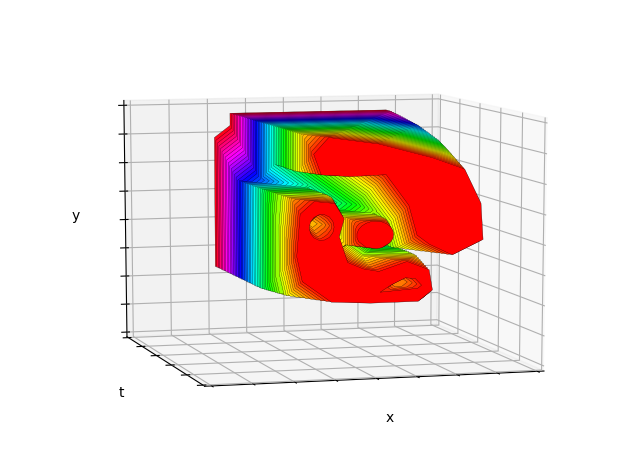
\includegraphics[width=\linewidth,height=0.8\textheight,keepaspectratio]{example3_bridge_front}
    \end{figure} 

  \end{frame}

  %----------------------------------------------------------------------------------------

  \begin{frame}
    \frametitle{Задача со сложным терминальным множеством мост сзади}

    \begin{figure}
        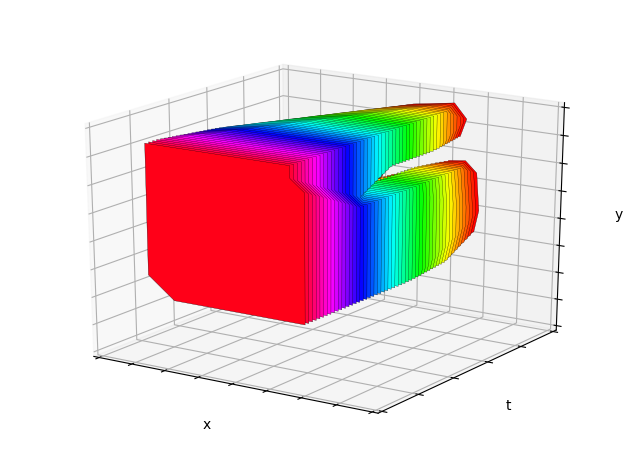
\includegraphics[width=\linewidth,height=0.8\textheight,keepaspectratio]{example3_bridge_back}
    \end{figure} 

  \end{frame}

  %----------------------------------------------------------------------------------------



  \begin{frame}
  \Huge{\centerline{Спасибо за внимание}}
  \end{frame}
  
  %----------------------------------------------------------------------------------------
  
  \end{document}